\section{Einleitung}

Die Interhyp AG ist Vermittler für private Baufinanzierungen. Das heißt, sie wählt aus einem Angebot von verschiedenen Darlehensgebern die optimale Finanzierungsstruktur für einen Kunden aus. Das Unternehmen wurde 1999 von den ehemaligen Goldman-Sachs-Bankern Robert Haselsteiner und Marcus Wolsdorf gegründet. Sechs Jahre später eröffnete die Interhyp AG erste Niederlassungen und konnte gleichzeitig den erfolgreichsten deutschen Börsengang des Jahres verzeichnen. Nach weiteren drei Jahren erfolgte die Übernahme durch ING DIRECT, der weltweilt größten und erfolgreichsten Direktbanken-Gruppe. Heute ist die Interhyp AG der größte Vermittler für private Baufinanzierungen in Deutschland, wurde acht mal in Folge als "Bester Baufinananzierer" (Zeitschrift \euro, Ausgabe 08/2013) ausgezeichnet und verfügt über mehr als 60 Beratungsstandorte mit über 1.000 Mitarbeitern.\\
Das primäre Ziel des Marketing der Interhyp AG ist die Kundenakquise. Da etwa 80\% aller Kundenanträge online abgeschickt werden, liegt der Fokus der Marketing-Abteilung auf dem Online-Marketing, das über verschiedene Kanäle verfügt. Beispiele sind Kooperationen mit anderen Unternehmen wie Immobilienscout24, bezahlte Anzeigen bei Suchmaschinen, Newsletter oder diverse Bannerschaltungen. Durch Online-Tracking können die Werbekontakte eines potentiellen Kunden mit der Interhyp AG zusammengefasst werden. So entsteht ein sogenannter Funnel, wie es in Abbildung \ref{customerJourney} skizziert ist. Jeder potentielle Kunde hat einen oder mehrere aufeinanderfolgende Kontaktpunkte, wobei jeder Kontaktpunkt die genaue Zeit des Kontaktes sowie die Art des Kontaktes, das heißt die Information über welche Kampagne es zu dem Kontakt kam, enthält. Am Ende eines jeden Funnels steht der Abbruch der Beobachtung oder im Idealfall das Ausfüllen eines Onlineantrages durch den Kunden.
\begin{figure}[H]
    \centering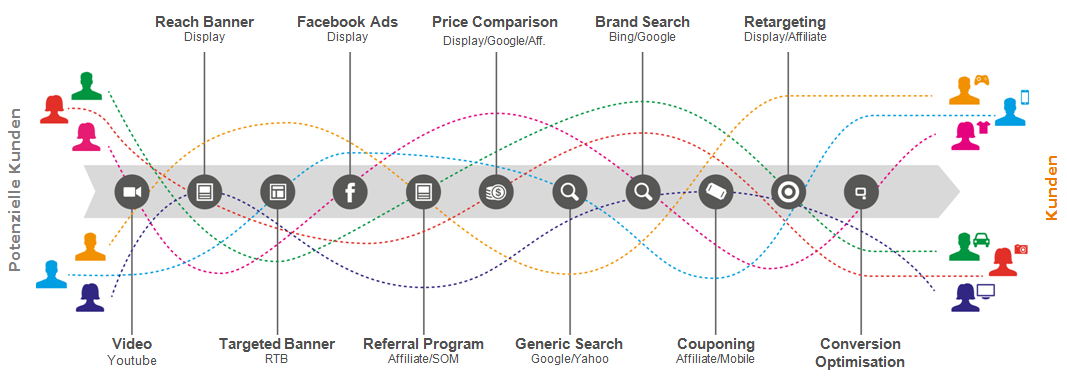
\includegraphics[scale=0.5]{customerJourney.png}\caption{Entstehung eines Funnels (Quelle: Interhyp AG)}\label{customerJourney}
\end{figure}
Die Refined Labs GmbH ist auf dem Gebiet des Online-Marketing spezialisiert und verantwortlich für das Online-Tracking der Werbekampagnen der Interhyp AG. Ein Funnel beginnt mit dem ersten Online-Werbekontakt eines potentiellen Kunden mit der Interhyp AG und der damit einhergehenden Erstellung eines Cookies. So können alle weiteren Werbekontakte dem potentiellen Kunden eindeutig zugewiesen werden. Das Tracking endet sobald der potentielle Kunde einen Onlineantrag versendet und damit zum Kunden wird. In diesem Fall spricht man von einem konvertierten Funnel. Wird innerhalb von $90$ Tagen kein Onlineantrag versendet, so wird das Cookie nicht weiter verfolgt und der Funnel wird als nicht-konvertiert bezeichnet.\\
Die Interhyp AG ist primär daran interessiert, ob man dem Abbruch eines Funnels entgegen wirken kann und damit allgemein an Unterschieden zwischen konvertierten und nicht-konvertierten Funnels. Um dieser Fragestellung gerecht zu werden, wurde ein zeitdiskretes Survival-Modell mittels Stochastic Gradient Boosting geschätzt und ein Sequential Pattern Mining-Algorithmus angewendet. Außerdem wurden die Funnels anhand eines Netzwerkes visualisiert.\\
Die Arbeit ist wie folgt gegliedert. In Kapitel \ref{datenlage} und \ref{descriptiv} werden die Datenaufbereitung und die Variablen erklärt. Daraufhin wird die Methodik des Survival-Modells in Kapitel \ref{survival}, der Sequential Pattern Mining-Algorithmus in Kapitel \ref{spm} und das Netzwerk in Kapitel \ref{network} erläutert. Die Ergebnisse dieser Methoden werden in Kapitel \ref{ergebnisse} vorgestellt und abschließend erfolgt eine Zusammenfassung in Kapitel \ref{zusammenfassung} und die Beschreibung des elektronischen Anhangs in Kapitel \ref{anhang}.